\documentclass[10pt]{beamer}

%% Chinese support
%% \usepackage[adobefonts,nocap]{ctex}

%% Fonts
\usepackage{multicol}
\usepackage{mathabx}
\usepackage[scaled]{helvet}
\usepackage{lmodern}
\usepackage{eulervm}
\usefonttheme[onlymath]{serif}
\usefonttheme{professionalfonts}
\usefonttheme{structurebold}
\usepackage{bm}
\usepackage{verbatim}

%% Color & Theme
\definecolor{SUblue}{RGB}{0,0,180}
\usecolortheme[RGB={0,0,180}]{structure}
\usetheme{Boadilla}
\setbeamertemplate{navigation symbols}{}
\setbeamertemplate{itemize items}[circle]
\setbeamertemplate{enumerate items}[circle]
\setbeamerfont{title}{size=\large}
\setbeamerfont{frametitle}{size=\large}
\setbeamerfont{framesubtitle}{size=\large,shape =$\color{violet}{\looparrowdownright}~$}
\setbeamercolor{title}{fg=white, bg= SUblue!75!green}
\setbeamercolor{framesubtitle}{fg=violet}
%\setlength{\leftmargini}{5pt}


\title[Statistical Computing]{{\textbf{Distribution and random numbers}}}

\author[Feng Li]{
\includegraphics[height=2cm]{cufelogo}\\
  \vspace{0.5cm}\textbf{Feng Li\\\texttt{feng.li@cufe.edu.cn}}}

\institute[Stat \& Math, CUFE]{\footnotesize{\textbf{School of
      Statistics and Mathematics\\ Central University of Finance and
      Economics}}}

\date{}
%%%%%%%%%%%%%%%%%%%%%%%%%%%%%%%%%%%%%%%%%%%%%%%%%%%%%%%%%%%%%%%%%%%%%%
\begin{document}

%% Title page
\begin{frame}[plain]
  \titlepage
  \tiny{Revised on \today}
\end{frame}


%% Outline page
\section*{Today we are going to learn...}
\begin{frame}
  \frametitle{Today we are going to learn...}
  \tableofcontents
\end{frame}


\section{Basic concepts of random numbers}
\begin{frame}
  \frametitle{Preliminary}

  \begin{itemize}

  \item \textbf{Pseudo random numbers}
    \begin{itemize}
    \item an algorithm for generating a sequence of numbers that
      approximates the properties of random numbers.

    \item The sequence is not truly random in that it is completely
      determined by a relatively small set of initial values, called
      the PRNG's state.

    \item Pseudo random numbers are important in practice for their
      \textbf{speed} in number generation and their
      \textbf{reproducibility}.

    \end{itemize}



  \item \textbf{Random seed}

    A random seed (or seed state, or just seed) is a number (or
    vector) used to initialize a pseudo random number generator.

  \item The most important random numbers are from uniform
    distributed numbers.

    \texttt{> runif(n,a,b)}

  \item Numbers selected from a non-uniform probability distribution
    can be generated using a uniform distribution PRNG and a function
    that relates the two distributions.


  \item Assume you have uniformly distributed random numbers from [0,
    1], how do you extend it to [a, b]?

  \end{itemize}
\end{frame}

\section{Continuous random variables}
\begin{frame}
\frametitle{Normal Distribution}

  \begin{itemize}
  \item \textbf{The normal density function}
    \begin{equation*}
    f(x, \mu, \sigma) = \frac{1}{\sigma\sqrt{2\pi}} e^{
      -\frac{(x-\mu)^2}{2\sigma^2} }
    \end{equation*}

    \texttt{> dnorm(x,mu,sigma)}

    \texttt{> dnorm(x,mu,sigma, log=TRUE)}


    \begin{itemize}
    \item In theory, \texttt{dnorm(x,mu,sigma,
        log=TRUE)==log(dnorm(x,mu,sigma))} but
      \texttt{dnorm(x,mu,sigma, log=TRUE)} but is more stable for very
      large values. Why?

    \item \textbf{We love logs}.
    \end{itemize}

  \item \textbf{The CDF} (cumulate desity function)
    \begin{equation*}
      \Phi(x)\;=\int_{-\infty}^x f(t, \mu, \sigma) d t
    \end{equation*}

    \texttt{> pnorm(q,mu,sigma)}


  \item \textbf{The quantile} (Given CDF, what is x?),
    i.e. $\Phi^{-1}(p)$

    \texttt{> qnorm(p,mu,sigma)}


  \item \textbf{Random numbers from normal distribution}

    \texttt{> rnorm(n,mu,sigma)}
  \end{itemize}

\end{frame}

\section{Likelihood Function}
\begin{frame}
  \frametitle{Likelihood function}

  \begin{itemize}
  \item Given that $x_i\sim N(\mu,\sigma)$ for $i=1,...,n$, the
    \textbf{likelihood function} is

    \begin{equation*}
      \prod_{i=1}^n f(x_i,\mu,\sigma)
    \end{equation*}

  \item However the \textbf{log likelihood function} is more often used
    \begin{equation*}
      \sum_{i=1}^n \log f(x_i,\mu,\sigma)
    \end{equation*}

  \item Do you know why?

  \end{itemize}
\end{frame}


\section{Walking APP example}

\begin{frame}
  \frametitle{How long do you walk every day?}

  \begin{itemize}
  \item Here is a list about my past six days walking statistics. Can you estimate how
    long do I walk everyday? and what is the variation?

  \end{itemize}

    \begin{figure}
      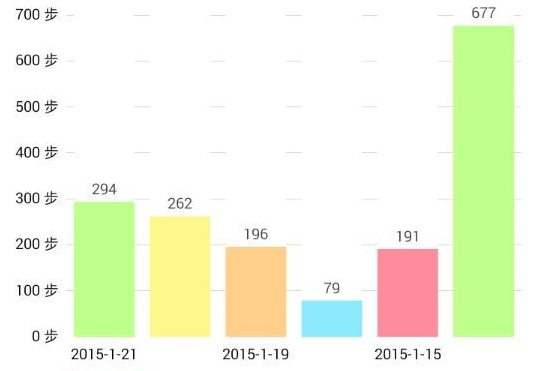
\includegraphics[width=0.7\textwidth]{walking2}
    \end{figure}

\end{frame}


\begin{frame}[fragile]
  \frametitle{The likelihood function}

  \begin{itemize}
  \item We assume everyday's walking steps ($x_i$) are independent, and  $x_i$ follows
    standard normal distribution $\sim
    N(\mu,\sigma)$, the corresponding likelihood function is

    \begin{equation*}
      \prod_{i=1}^n f(x_i,\mu,\sigma)
    \end{equation*}

    which can be easily written in R as
\begin{verbatim}
logNormLike <- function(mu, sigma, data)
  {
    out = sum(dnorm(x = data, mean = mu, sd = sigma,log = TRUE))
    return(out)
  }
\end{verbatim}


  \item \textbf{The scope} Find a proper combination of $\mu$ and $\sigma$ that maximizes the
    loglikelihood function.

  \end{itemize}
\end{frame}


\begin{frame}[allowframebreaks]
  \frametitle{Conditional likelihood function}

  \begin{itemize}
  \item Fix other parameters
    \begin{figure}
      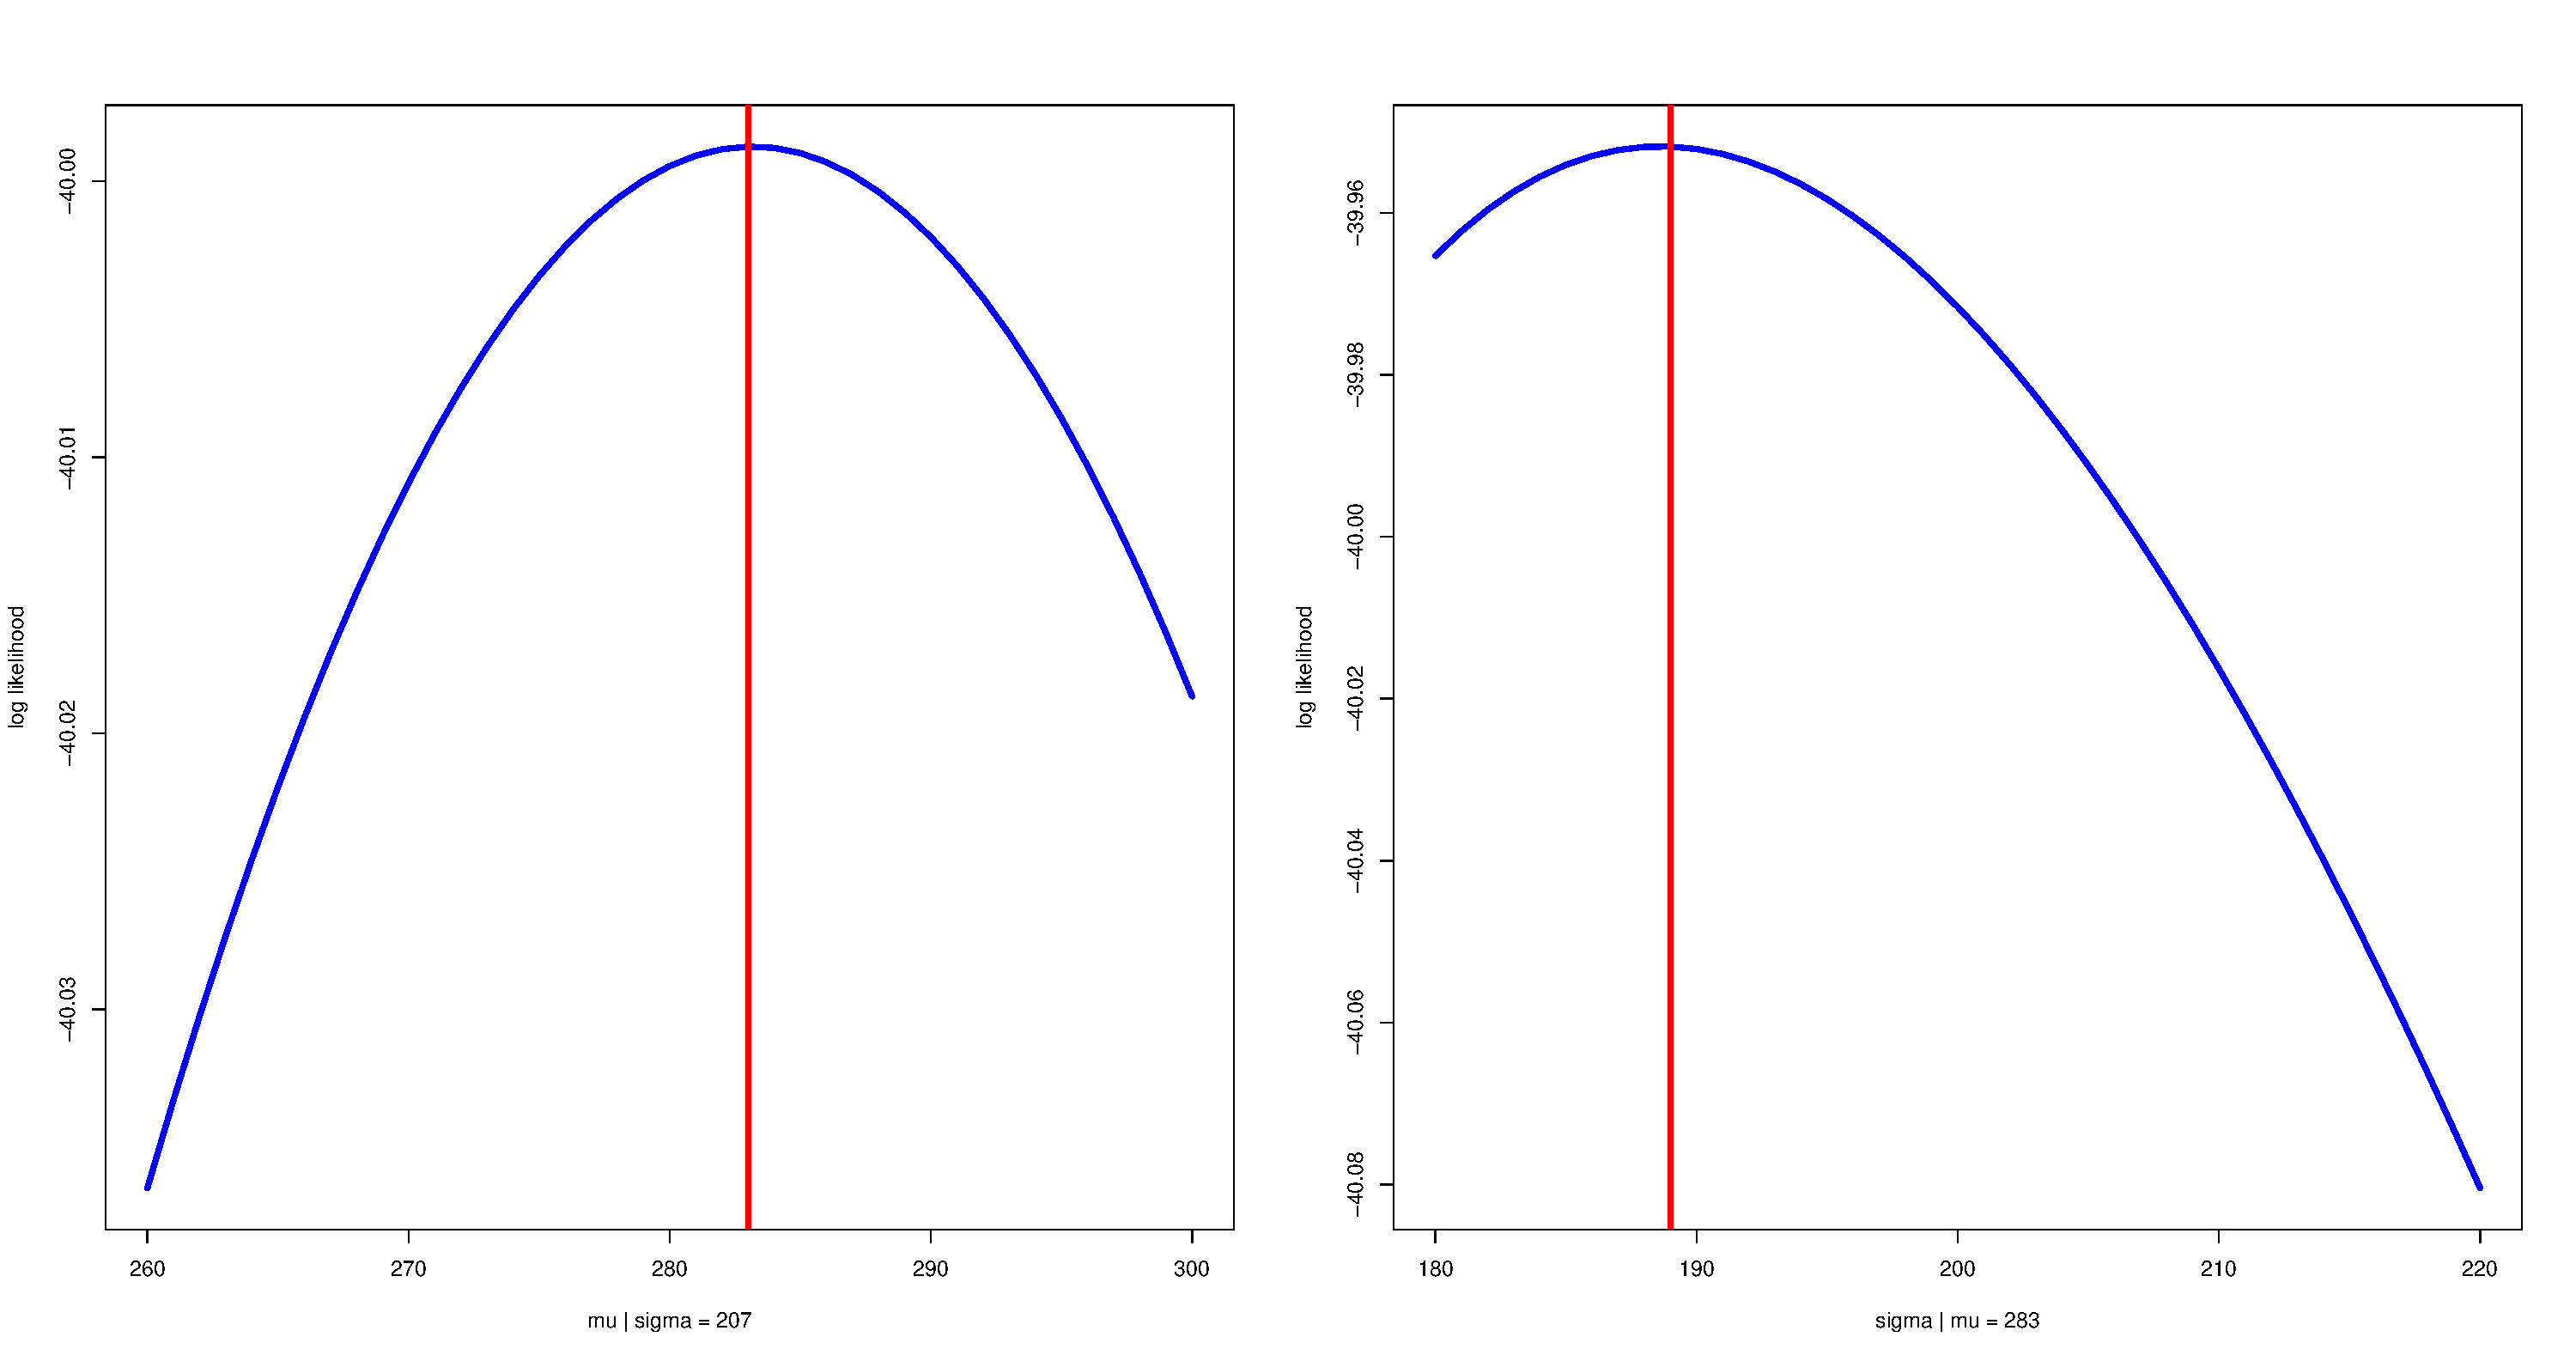
\includegraphics[width=0.7\textwidth]{conddesity}
%      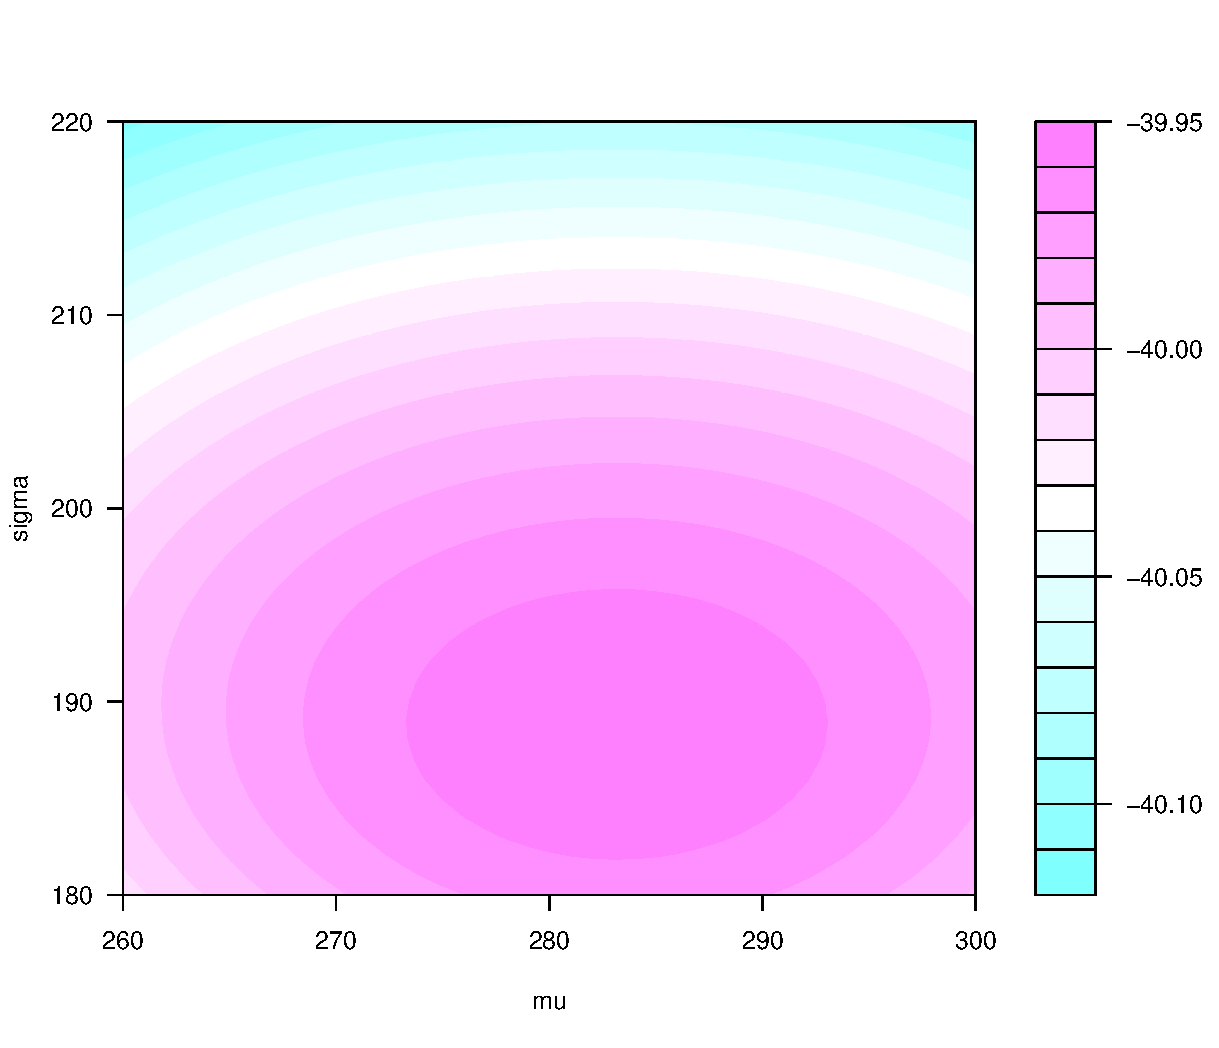
\includegraphics[width=0.5\textwidth]{2dlike}
      \caption{Left: fix variance to allow $\mu$ to change with likelihood
        function. Right: fix mean to allow $\sigma$ to change with likelihood function.}
    \end{figure}

  \item  Are $\mu$ and $\sigma$ we obtained the best combination?

%   \end{itemize}

% \end{frame}


% \begin{frame}
%   \frametitle{利用牛顿迭代求解极大似然函数}

%   \begin{itemize}
%   \item 对数似然函数的一阶和二阶偏导的解析解
%     \begin{align*}
%      L'(\mu)=\sum_{i=1}^n \frac{\partial \log f(x_i,\mu,\sigma)}{\partial \mu},
%       L'(\sigma)=\sum_{i=1}^n \frac{\partial \log f(x_i,\mu,\sigma)}{\partial \sigma}\\
% \\
%       L''(\mu)=\sum_{i=1}^n \frac{\partial^2 \log f(x_i,\mu,\sigma)}{\partial \mu^2},     L''(\sigma)=\sum_{i=1}^n \frac{\partial^2 \log f(x_i,\mu,\sigma)}{\partial \sigma^2}
%     \end{align*}


% \item 按照以下交互迭代直到收敛
%     \begin{align*}
%       \mu_{t+1} = \mu_t - \left(L''(\mu)\right)^{-1} L'(\mu) \mid_{\mu=\mu_t, \sigma=\sigma_t}\\
%      \sigma_{t+1} = \sigma_t - \left(L''(\sigma)\right)^{-1} L'(\sigma)
%       \mid_{\sigma=\sigma_t, \sigma=\sigma_t}
%     \end{align*}

%   \item \textbf{思考}: 为什么要交互迭代?可不可以将其中一个参数迭代收敛后再迭代其他的参数?

%   \end{itemize}



%     \begin{figure}
%       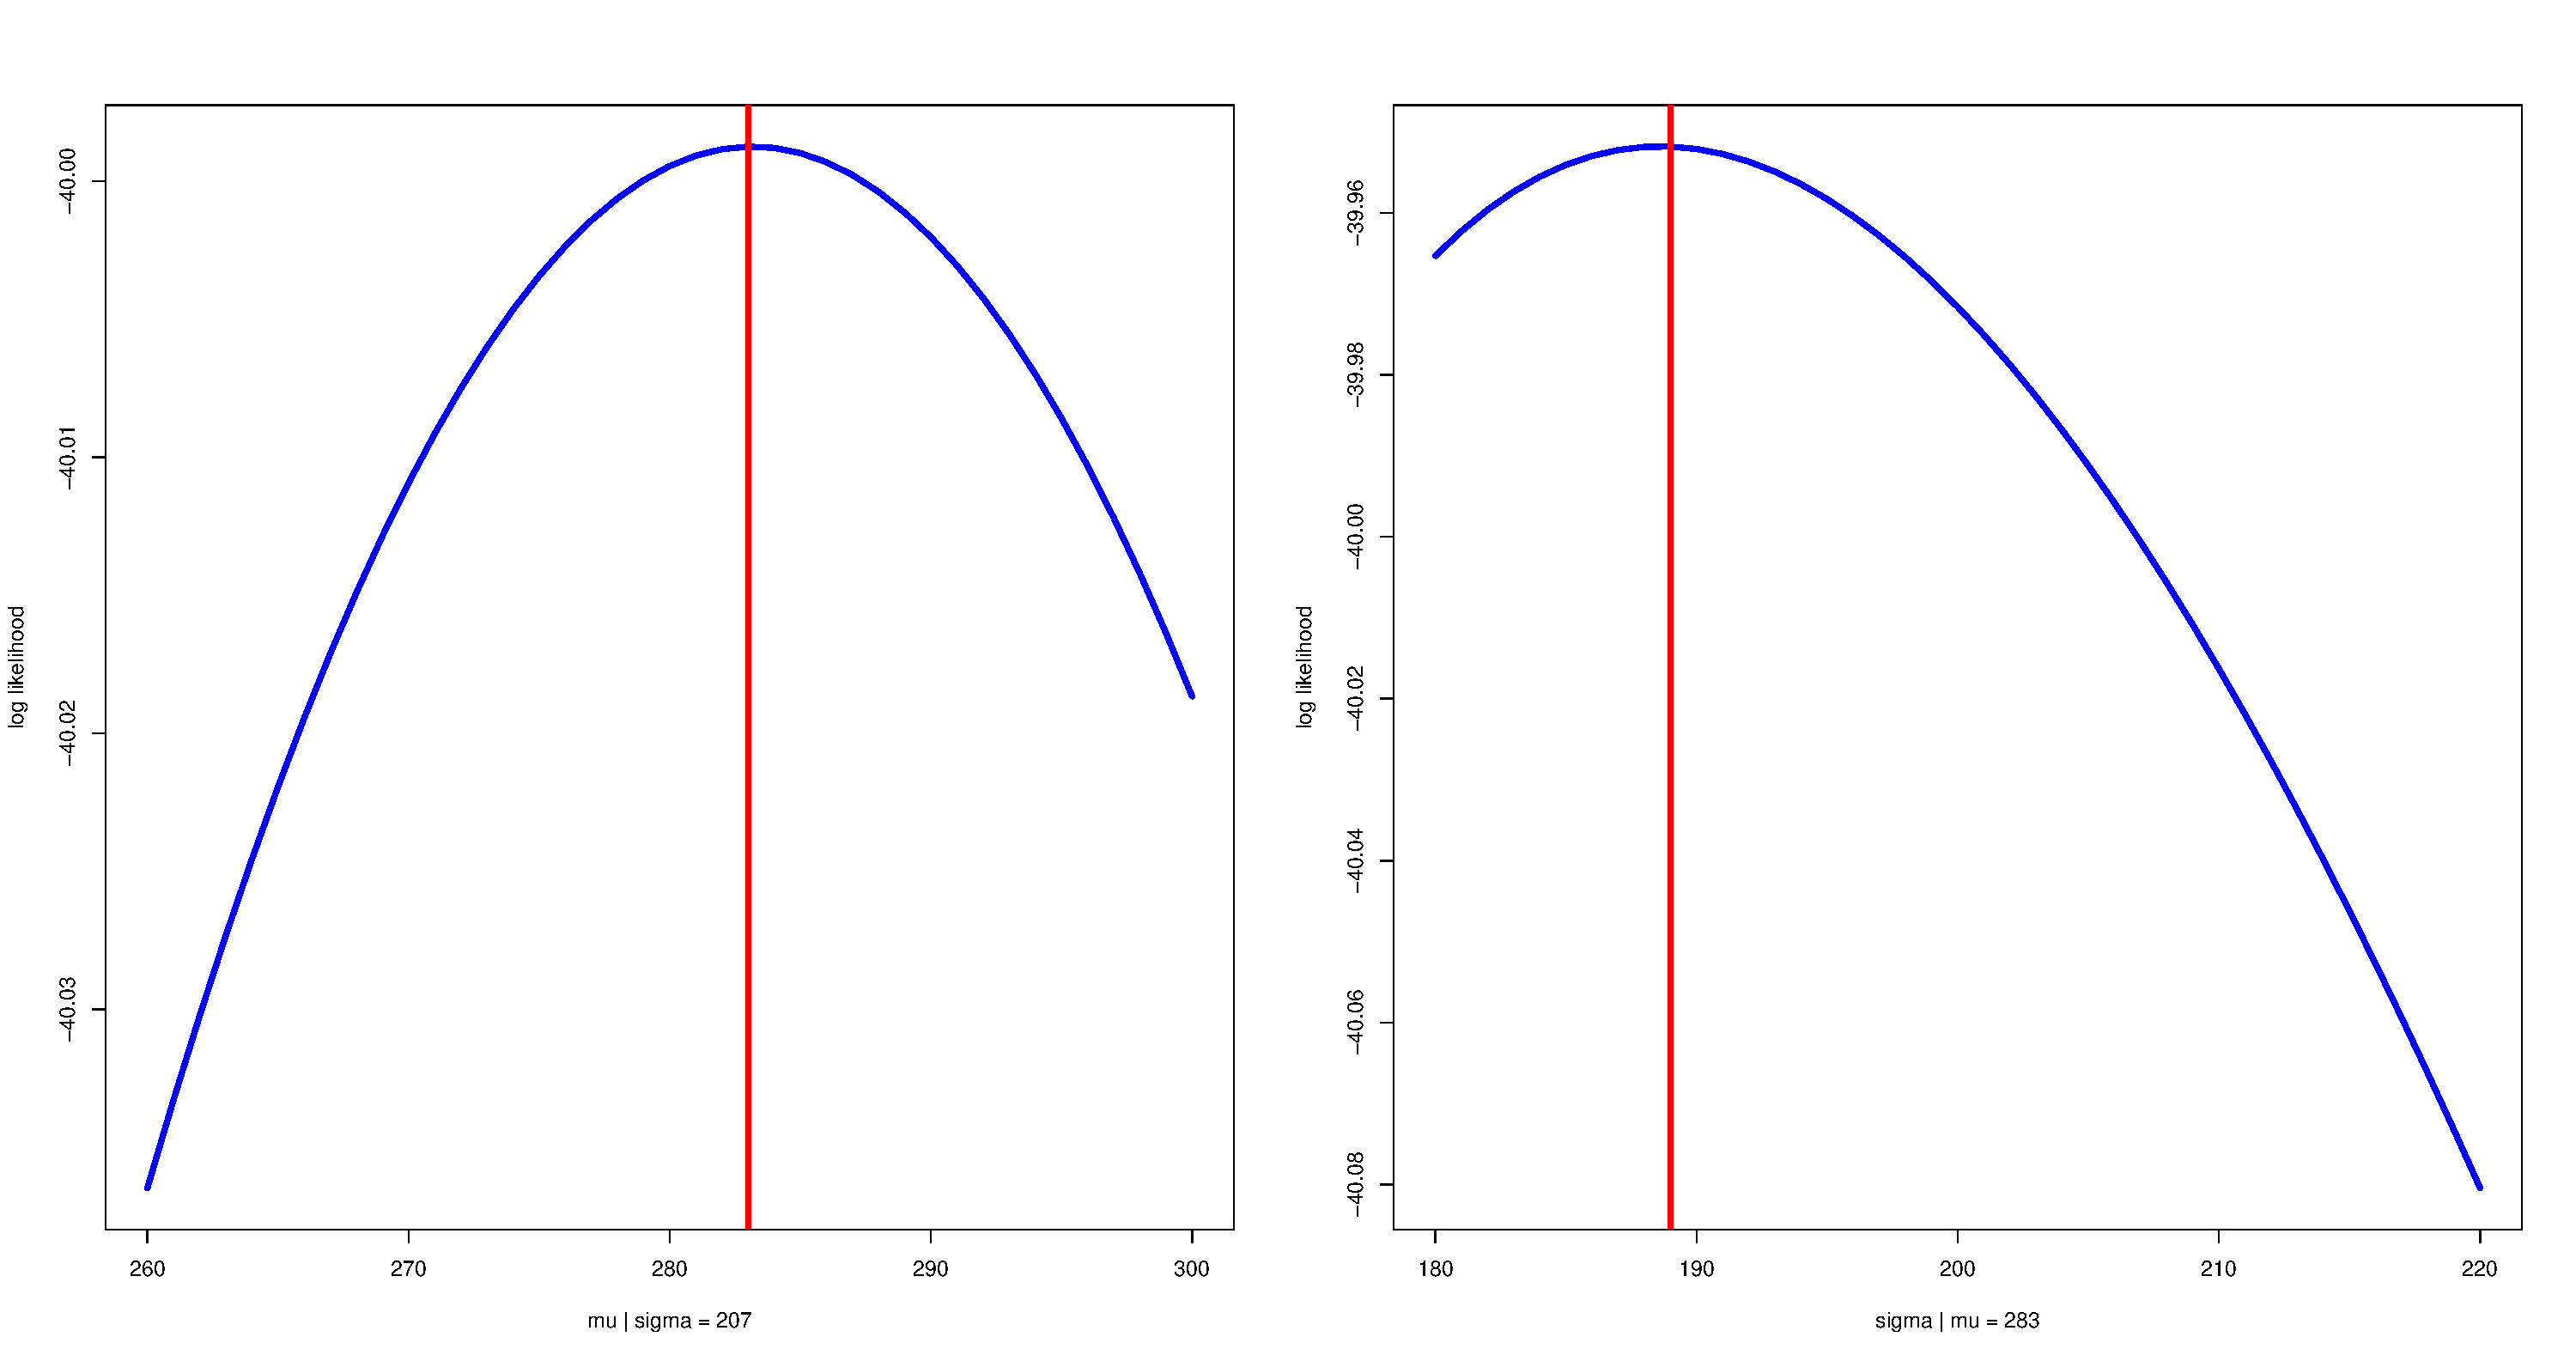
\includegraphics[width=1\textwidth]{conddesity}
% %      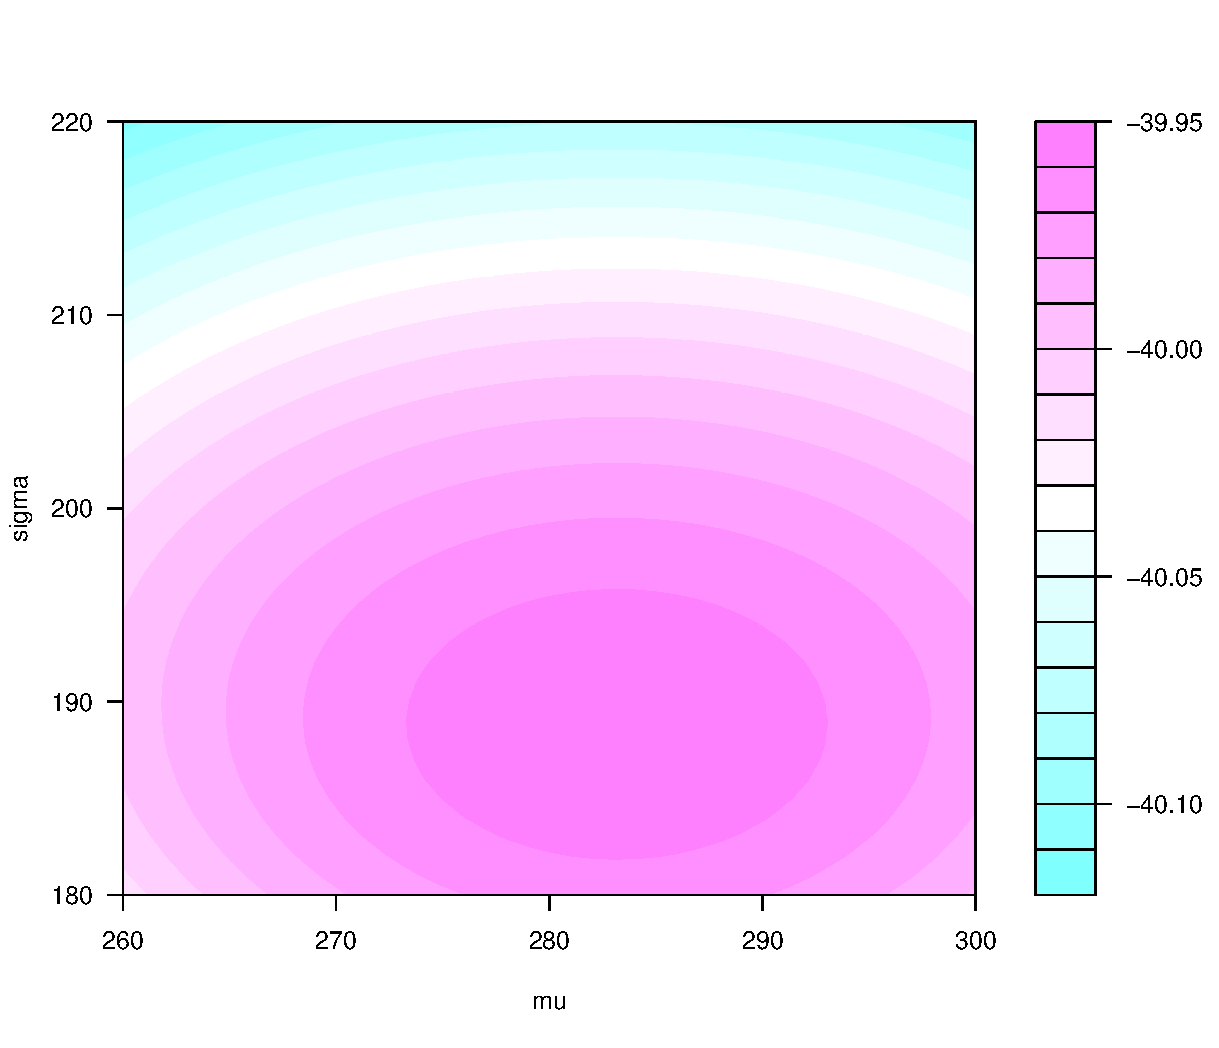
\includegraphics[width=0.5\textwidth]{2dlike}
%       \caption{左图:给定方差对数似然函数随$\mu$的变化而变化,右图:给定均值对数似然函数
%         随$\sigma$的变化而变化。}
%     \end{figure}

% \end{frame}

% \begin{frame}
%   \frametitle{通过牛顿迭代似然函数如何随参数的变化而变化}


%   \begin{itemize}
%   \item 利用牛顿迭代对我们健走的数据进行似然估计
    \newpage
    \begin{figure}
      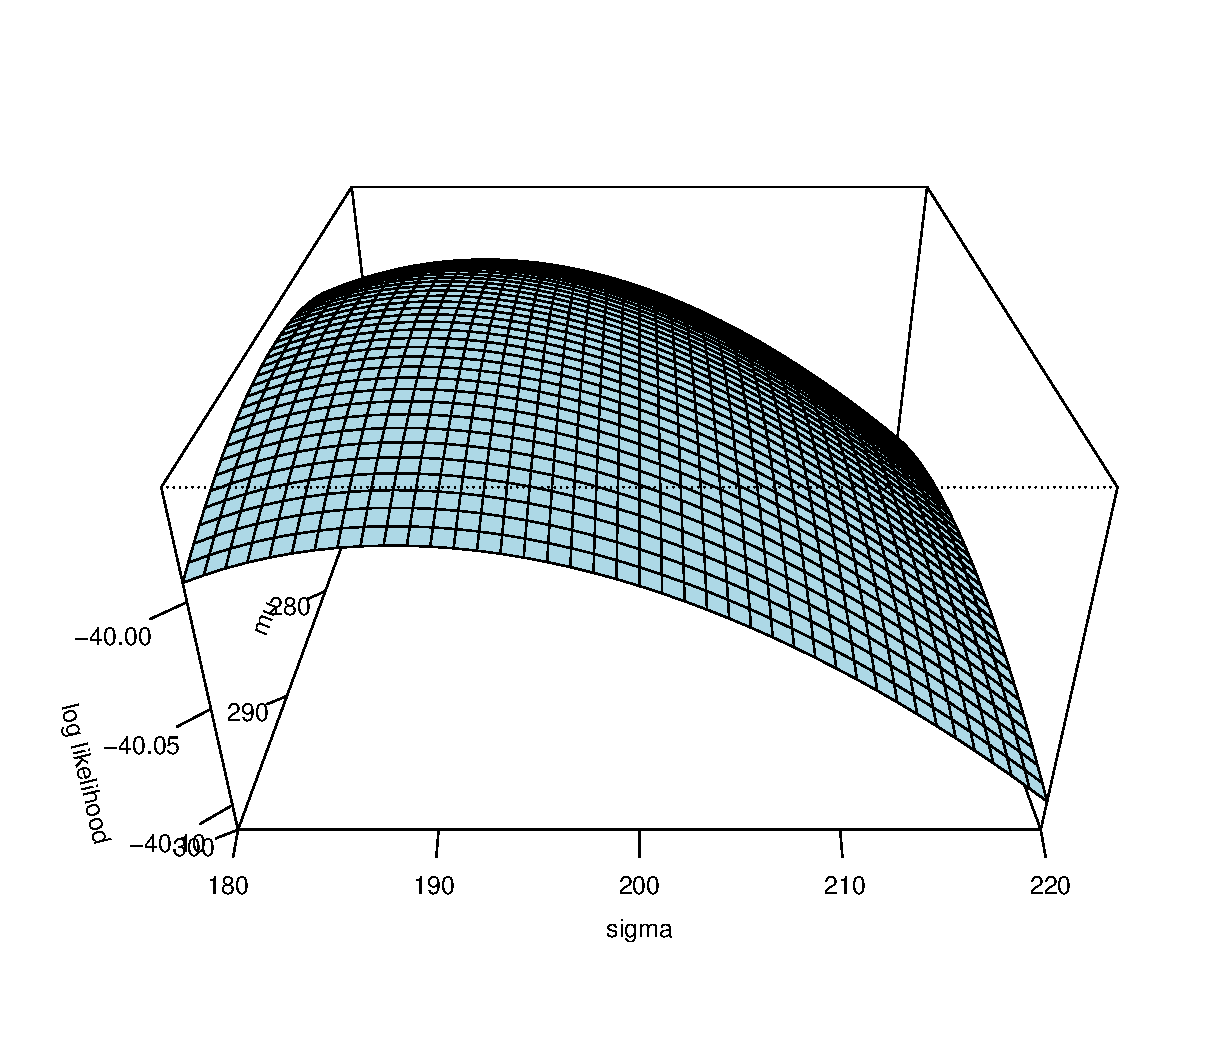
\includegraphics[width=0.45\textwidth]{3dlike}
      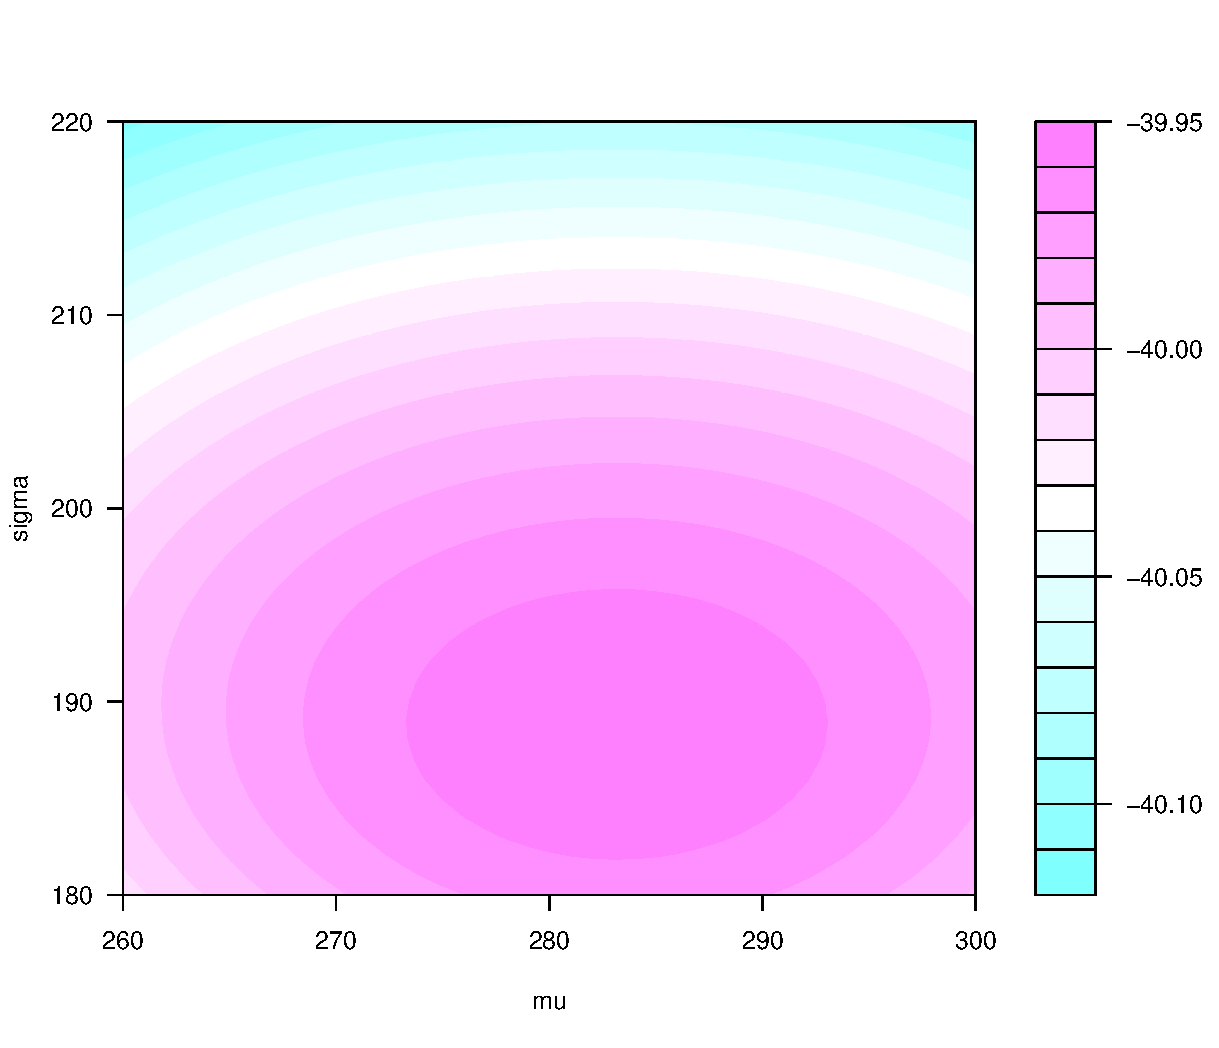
\includegraphics[width=0.45\textwidth]{2dlike}
      \caption{2D and 3D loglikelihood function}
    \end{figure}

  % \item 当$\mu=285,\sigma=191$时,我们的对数似然函数达到极大值$-39.95$。

  \end{itemize}

\end{frame}


% \section{课后思考}


% \begin{frame}
% \frametitle{课后思考}
% \begin{itemize}
% \item 在健走示例中我们的假设有何问题?

% \item 通过极大似然估计得到的均值和方差和我们直接对样本求均值和方差所得到的结果是一定吻合的
%   吗?


% \end{itemize}

% \end{frame}



\begin{frame}
  \frametitle{Likelihood function for linear regression}
  \begin{itemize}
  \item Assume you want to make a regression model

    \begin{equation*}
      y_i = \beta_0 + \beta_1 x_i + \epsilon_i
    \end{equation*}

    where $\epsilon_i \sim N(0, \sigma^2)$

  \item What is the (log) likelihood function?

  \item What are the unknown parameters?

  \item How do we estimate the parameters?


    \begin{itemize}
    \item Write down a likelihood function with respect to the
      unknown parameters.

    \item Use an optimization algorithm to find the estimates of the
      unknown parameters.

    \end{itemize}

  \end{itemize}

\end{frame}

\begin{frame}[fragile]
\frametitle{The Likelihood function}

\begin{verbatim}
logNormLikelihood <- function(par, y, x)
    {
        beta0 <- par[1]
        beta1 <- par[2]
        sigma <- par[3]

        mean <- beta0 + x*beta1

        logDens <- dnorm(x = y, mean = mean,
                         sd = sigma, log = TRUE)
        loglikelihood <- sum(logDens)

        return(loglikelihood)
    }
\end{verbatim}

\end{frame}


\begin{frame}[fragile]
  \frametitle{Other types of continuous distribution}

\begin{itemize}
\item

\begin{verbatim}
Distribution                 Function in R
------------------------------------------
Student t                    {p,d,q}t
Chi squared                  {p,d,q}chi
Gamma                        {p,d,q}gamma
Exponential                  {p,d,q}exp
------------------------------------------
\end{verbatim}

\item For a significance test, what distribution do you use?

\end{itemize}
\end{frame}

\section{Discrete random variables}

\begin{frame}[fragile]
\frametitle{Discrete random variables}
\begin{itemize}
\item

\begin{verbatim}
Distribution                 Function in R
------------------------------------------
Binomial                     {p,d,q}binorm
Negative binomial            {p,d,q}nbinom
Poisson                      {p,d,q}pois
Geometric                    {p,d,q}geom
------------------------------------------
\end{verbatim}

\item Bernoulli distribution is a special case of binomial distribution.

\end{itemize}
\end{frame}

\begin{frame}
  \frametitle{Suggested reading}

  \begin{itemize}
  \item Jones (2009): \textbf{Chapter 14, 15, 16}
  \end{itemize}

\end{frame}


\end{document}
